
{{\setbeamertemplate{background canvas}{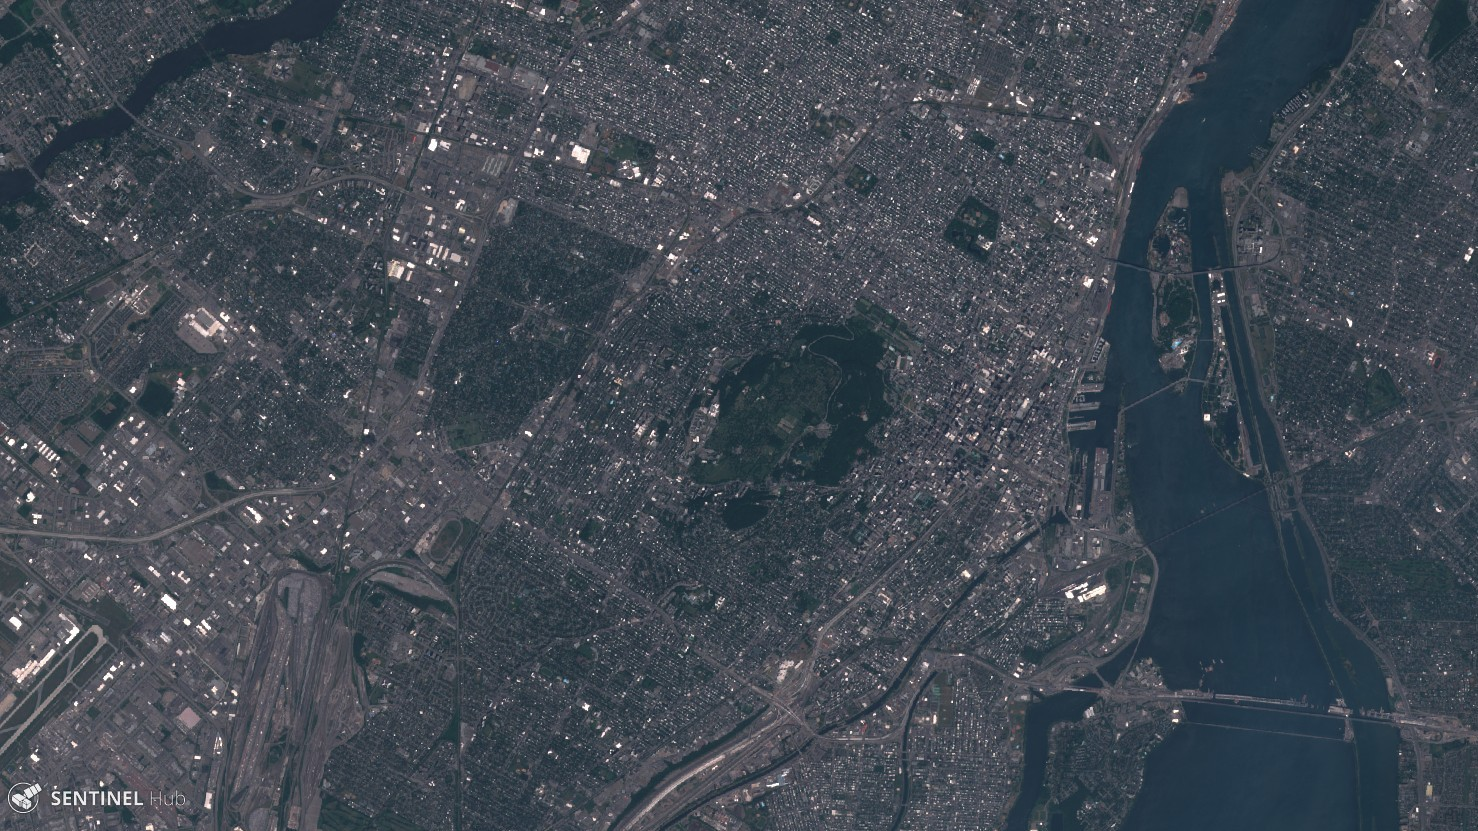
\includegraphics[width=\paperwidth]{images/cloudfree}}
\begin{frame}[plain, b]
%\frametitle{When we think of satellite images we picture this}
%%\centering\includegraphics[width=.75\textwidth]{images/montreal_satellite}
%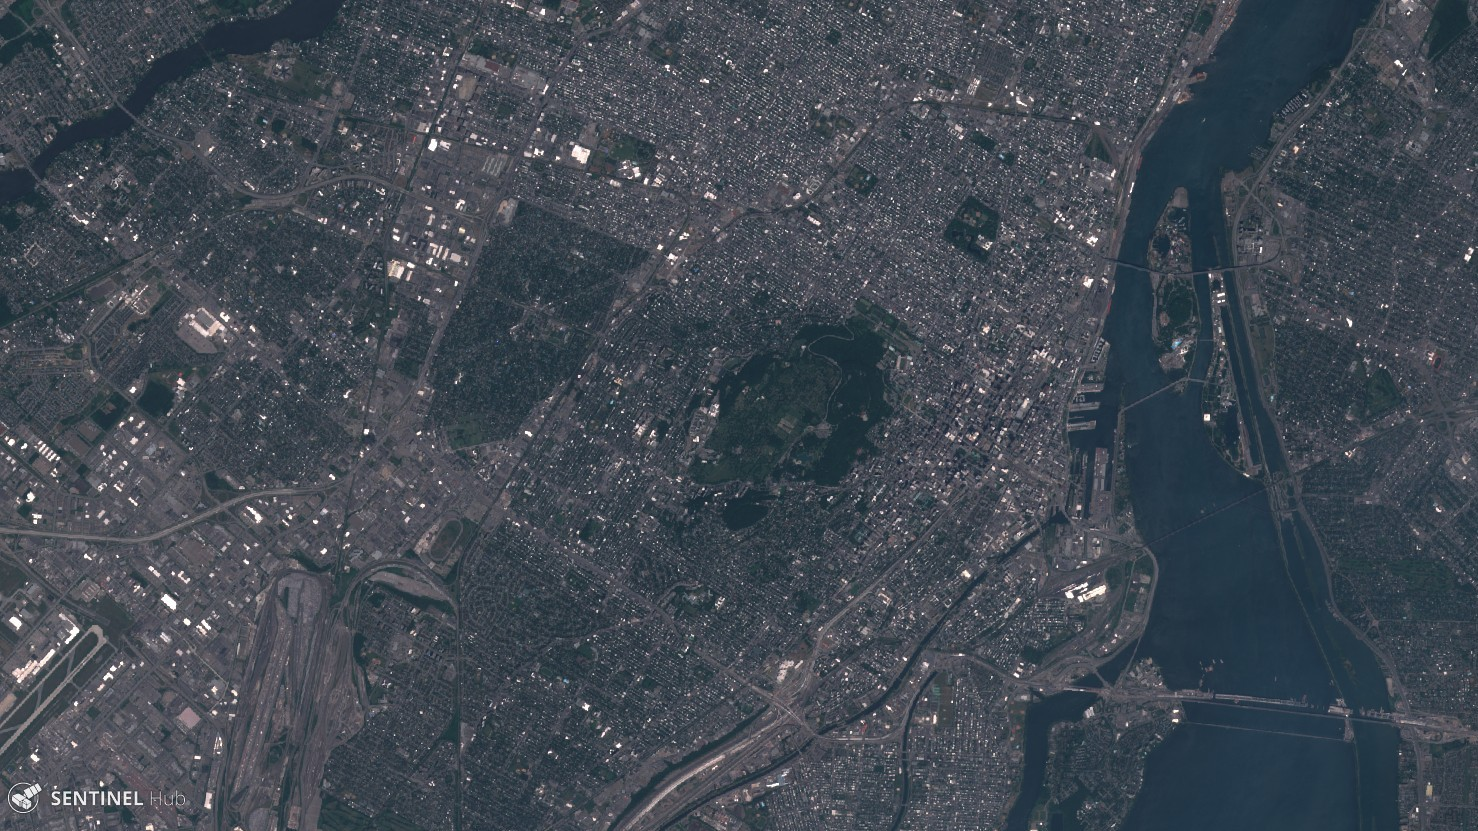
\includegraphics[width=\textwidth]{images/cloudfree}


	\raggedleft \color{white} Montréal, 2018
\end{frame}
}

{\setbeamertemplate{background canvas}{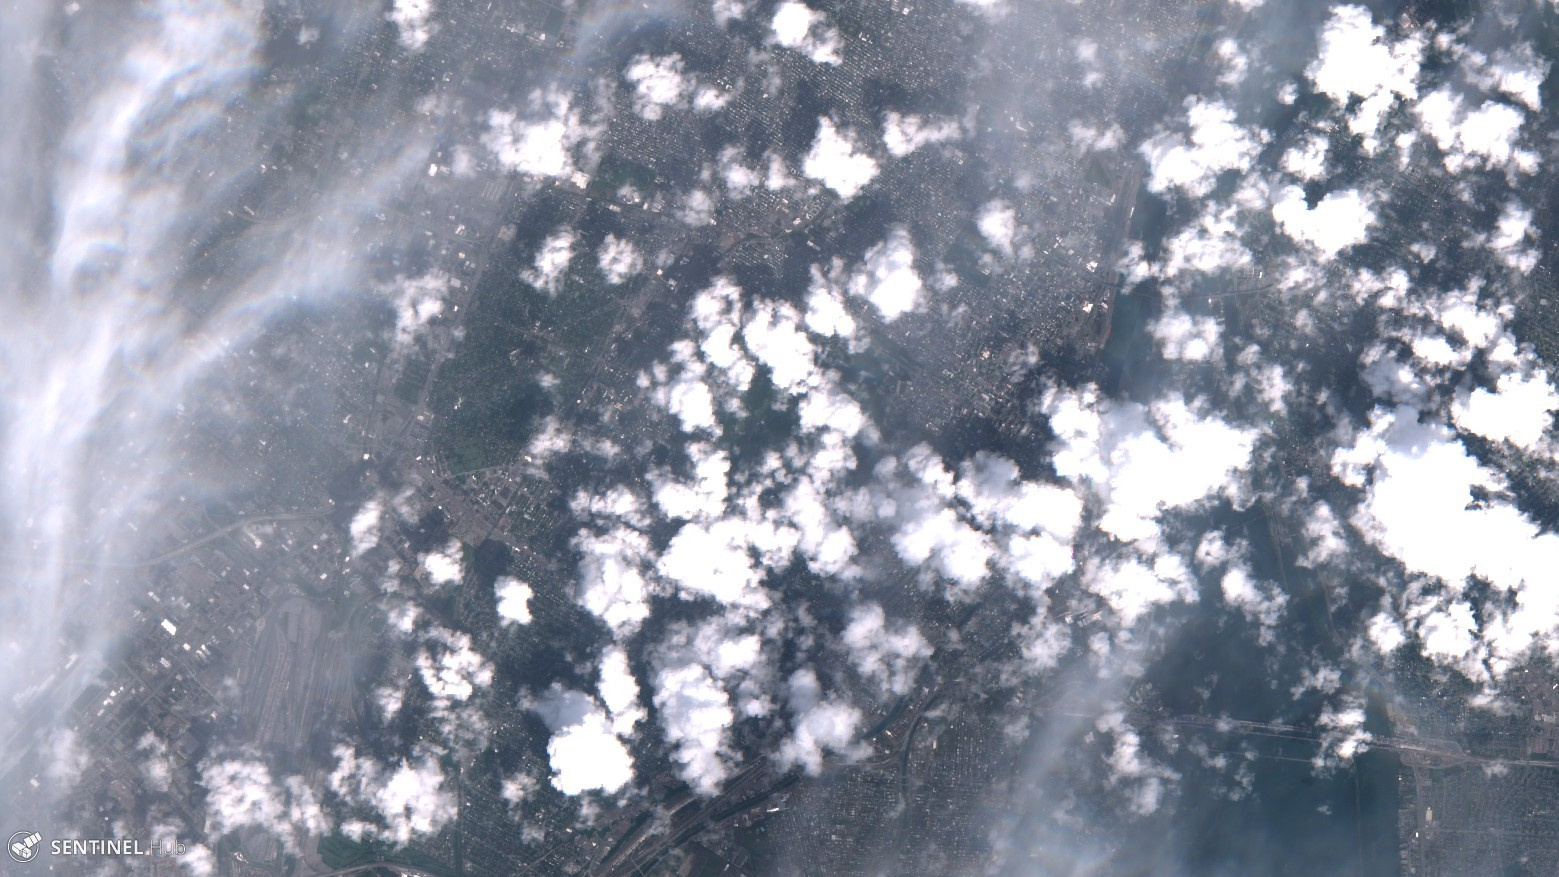
\includegraphics[width=\paperwidth]{images/clouds}}
	\begin{frame}[plain, b]
%		\frametitle{... however, ususally }
			
		\raggedleft \color{white} Montréal, 2018
	%		\includegraphics[width=\textwidth]{images/cloud_airplane}
			
	\end{frame}
	
}

%{\setbeamercolor{background canvas}{bg=tumbluedark}
%	\begin{frame}[plain]
%	
%	\vspace{8em}
%	\begin{center}
%		\Huge\color{tumwhite}
%		How should we deal with $
\includegraphics[width=2em]{images/icons/cloud2}^\ast$?
%	\end{center}\color{white}
%	\vspace{2em}
%	\raggedleft \Large$^\ast$ ...and other noise in the data
%	
%	\vfill
%	\vspace{6em}
%	\raggedleft{\small \color{tumgray}
%	Icons made by Smashicons from www.flaticon.com
%	}
%\end{frame}
%}


\begin{frame}<presentation:1>
\frametitle{Cloud coverage}
\centering

\def\imagewidth{1.5cm}


\visible<1>{\includegraphics[width=\imagewidth]{images/activations/16494/x/x-0.png}}
\visible<1>{\includegraphics[width=\imagewidth]{images/activations/16494/x/x-1.png}}
\visible<1>{\includegraphics[width=\imagewidth]{images/activations/16494/x/x-2.png}}
\visible<1>{\includegraphics[width=\imagewidth]{images/activations/16494/x/x-3.png}}
\visible<1>{\includegraphics[width=\imagewidth]{images/activations/16494/x/x-4.png}}
\visible<1,2>{\includegraphics[width=\imagewidth]{images/activations/16494/x/x-5.png}}
\visible<1>{\includegraphics[width=\imagewidth]{images/activations/16494/x/x-6.png}}
\visible<1>{\includegraphics[width=\imagewidth]{images/activations/16494/x/x-7.png}}
\visible<1,2>{\includegraphics[width=\imagewidth]{images/activations/16494/x/x-8.png}}
\visible<1>{\includegraphics[width=\imagewidth]{images/activations/16494/x/x-9.png}}
\visible<1>{\includegraphics[width=\imagewidth]{images/activations/16494/x/x-10.png}}
\visible<1>{\includegraphics[width=\imagewidth]{images/activations/16494/x/x-11.png}}
\visible<1,2>{\includegraphics[width=\imagewidth]{images/activations/16494/x/x-12.png}}
\visible<1,2>{\includegraphics[width=\imagewidth]{images/activations/16494/x/x-13.png}}
\visible<1,2>{\includegraphics[width=\imagewidth]{images/activations/16494/x/x-14.png}}
\visible<1,2>{\includegraphics[width=\imagewidth]{images/activations/16494/x/x-15.png}}
\visible<1,2>{\includegraphics[width=\imagewidth]{images/activations/16494/x/x-16.png}}
\visible<1>{\includegraphics[width=\imagewidth]{images/activations/16494/x/x-18.png}}
\visible<1>{\includegraphics[width=\imagewidth]{images/activations/16494/x/x-19.png}}
\visible<1,2>{\includegraphics[width=\imagewidth]{images/activations/16494/x/x-20.png}}
\visible<1,2>{\includegraphics[width=\imagewidth]{images/activations/16494/x/x-21.png}}
\visible<1>{\includegraphics[width=\imagewidth]{images/activations/16494/x/x-22.png}}
\visible<1>{\includegraphics[width=\imagewidth]{images/activations/16494/x/x-23.png}}
\visible<1>{\includegraphics[width=\imagewidth]{images/activations/16494/x/x-24.png}}
\visible<1>{\includegraphics[width=\imagewidth]{images/activations/16494/x/x-25.png}}
\visible<1>{\includegraphics[width=\imagewidth]{images/activations/16494/x/x-26.png}}
\visible<1,2>{\includegraphics[width=\imagewidth]{images/activations/16494/x/x-27.png}}
\visible<1>{\includegraphics[width=\imagewidth]{images/activations/16494/x/x-28.png}}
\visible<1,2>{\includegraphics[width=\imagewidth]{images/activations/16494/x/x-29.png}}
\visible<1>{\includegraphics[width=\imagewidth]{images/activations/16494/x/x-30.png}}
\visible<1>{\includegraphics[width=\imagewidth]{images/activations/16494/x/x-31.png}}
\visible<1,2>{\includegraphics[width=\imagewidth]{images/activations/16494/x/x-32.png}}
\visible<1>{\includegraphics[width=\imagewidth]{images/activations/16494/x/x-33.png}}
%	
\end{frame}

\newcommand{\xtvector}{
	\begin{tikzpicture}[baseline=-1.9em,yscale=-5]
		\node[draw=tumgraylight, circle, fill=b2color, text=white, text opacity=1, font=\small, inner sep=.1em](d) at (0,0){};
		\node[draw=tumgraylight, circle, fill=b3color, text=white, text opacity=1, font=\small, inner sep=.1em](d) at (0,1){};
		\node[draw=tumgraylight, circle, fill=b4color, text=white, text opacity=1, font=\small, inner sep=.1em](d) at (0,2){};
		\node[draw=tumgraylight, circle, fill=b5color, text=white, text opacity=1, font=\small, inner sep=.1em](d) at (0,3){};
		\node[draw=tumgraylight, circle, fill=b6color, text=white, text opacity=1, font=\small, inner sep=.1em](d) at (0,4){};
		\node[draw=tumgraylight, circle, fill=b7color, text=white, text opacity=1, font=\small, inner sep=.1em](d) at (0,5){};
		\node[draw=tumgraylight, circle, fill=b8color, text=white, text opacity=1, font=\small, inner sep=.1em](d) at (0,6){};
		\node[draw=tumgraylight, circle, fill=b8Acolor, text=white, text opacity=1, font=\small, inner sep=.1em](d) at (0,7){};
		\node[draw=tumgraylight, circle, fill=b11color, text=white, text opacity=1, font=\small, inner sep=.1em](d) at (0,8){};
		\node[draw=tumgraylight, circle, fill=b12color, text=white, text opacity=1, font=\small, inner sep=.1em](d) at (0,9){};
	\end{tikzpicture}
}



\begin{frame}
	\frametitle{Satellite Time Series}
	\framesubtitle{Sentinel 2 (raw), mean-aggregated pixels of a meadow field parcel}
	
	
	
	
	
	\begin{tikzpicture}[baseline=-2em, inner sep=0]
		
		\begin{axis}[
		width=\textwidth,
	%	hide axis,
		height=5.5cm,
		ymin=0, ymax=1.2,
		%no marks,  
		draw opacity=.8,
		smooth=0.001,
		legend style={at={(1,1.3)},line width=2pt, draw opacity=1},
		legend columns=5,
		ylabel={reflectance},
		xlabel={time $t$ {\small (January to December 2018)}}
		]
		
		
			\addplot[b2color, tsmark] table [x=t, y=B02, col sep=comma] {images/example/12-71456800_raw.csv};
			\addplot[b3color, tsmark] table [x=t, y=B03, col sep=comma] {images/example/12-71456800_raw.csv};
			\addplot[b4color, tsmark] table [x=t, y=B04, col sep=comma] {images/example/12-71456800_raw.csv};
			
			\only<2-3>{
				 \coordinate(c1) at (axis cs:15,1.1);
				 \coordinate(c2) at (axis cs:10,.8);
				 \coordinate(c3) at (axis cs:0,.6);
				 \coordinate(c4) at (axis cs:40,.6);
				 \coordinate(c5) at (axis cs:46,.6);
%				 \coordinate(c6) at (axis cs:0,.6);
				 
				 \coordinate(c8) at (axis cs:24,.9);
				 \coordinate(c9) at (axis cs:27,.8);
				 \coordinate(c7) at (axis cs:29,.9);
				 
				 
				 \node[inner sep=.5em](annotclouds) at (axis cs:32,1.2){clouds};
				 \draw[-stealth] (annotclouds) -- (c7);
				 \draw[-stealth] (annotclouds) -- (c8);
				 \draw[-stealth] (annotclouds) -- (c9);
				 \draw[-stealth] (annotclouds) -- (c4);
				 \draw[-stealth] (annotclouds) -- (c5);
				 \draw[-stealth] (annotclouds) -- (c1);
%				 \draw[-stealth] (annotclouds) -- (c6);
				 
			}
			\only<3-3>{
				
				\node[inner sep=.5em](annotground) at (axis cs:47,1.2){ground};
				\coordinate(g1) at (axis cs:4,.2);
				\coordinate(g2) at (axis cs:8,.2);
				\coordinate(g3) at (axis cs:13,.2);
				\coordinate(g4) at (axis cs:18,.2);
				\coordinate(g5) at (axis cs:23,.2);
				\coordinate(g6) at (axis cs:31,.2);
				\coordinate(g7) at (axis cs:35,.2);
				\coordinate(g8) at (axis cs:41,.2);
				\coordinate(g9) at (axis cs:47,.2);
				
%				\draw[-stealth] (annotground) -- (g1);
%				\draw[-stealth] (annotground) -- (g2);
%				\draw[-stealth] (annotground) -- (g3);
%				\draw[-stealth] (annotground) -- (g4);
%				\draw[-stealth] (annotground) -- (g5);
				\draw[-stealth] (annotground) -- (g6);
				\draw[-stealth] (annotground) -- (g7);
				\draw[-stealth] (annotground) -- (g8);
				\draw[-stealth] (annotground) -- (g9);
				
			}
			
			\only<1->{
			\addplot[b5color, tsmark] table [x=t, y=B05, col sep=comma] {images/example/12-71456800_raw.csv};
			\addplot[b6color, tsmark] table [x=t, y=B06, col sep=comma] {images/example/12-71456800_raw.csv};
			\addplot[b7color, tsmark] table [x=t, y=B07, col sep=comma] {images/example/12-71456800_raw.csv};
			\addplot[b8color, tsmark] table [x=t, y=B08, col sep=comma] {images/example/12-71456800_raw.csv};
			\addplot[b8Acolor, tsmark] table [x=t, y=B8A, col sep=comma] {images/example/12-71456800_raw.csv};
			
			\addplot[b11color, tsmark] table [x=t, y=B11, col sep=comma] {images/example/12-71456800_raw.csv};
			\addplot[b12color, tsmark] table [x=t, y=B12, col sep=comma] {images/example/12-71456800_raw.csv};
			}
		
			\only<1-3>
			\legend{B02 (blue),B03 (green),B04 (red),B05,B06,B07,B08,B8A,B11,B12}
			
		\end{axis}
		
	\end{tikzpicture}
	
\end{frame}
